\documentclass{standalone}
\usepackage{tikz}
\usetikzlibrary{patterns, positioning}


\begin{document}
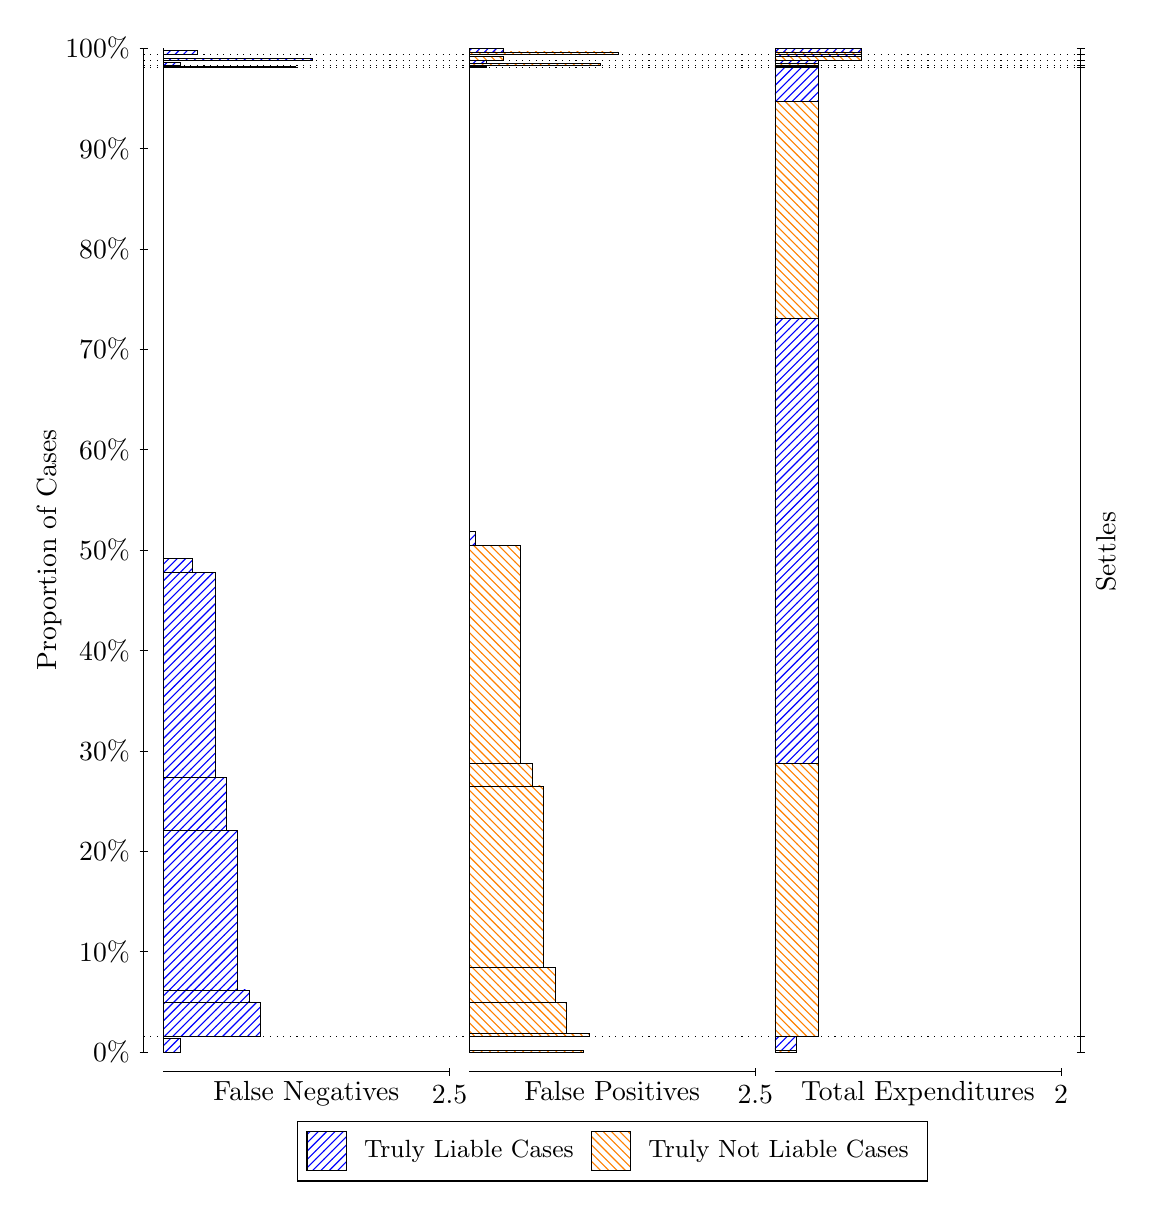
\begin{tikzpicture}
\draw[black, very thin] (1.5,1.75) -- (1.5,14.5);
\node[rotate=90, text=black, anchor=center] at (0.3, 8.125) {Proportion of Cases};
\draw[black, very thin] (1.45,1.75) -- (1.55,1.75);
\node[text=black, anchor=east] at (1.45, 1.75) {0\%};
\draw[black, very thin] (1.45,3.025) -- (1.55,3.025);
\node[text=black, anchor=east] at (1.45, 3.025) {10\%};
\draw[black, very thin] (1.45,4.3) -- (1.55,4.3);
\node[text=black, anchor=east] at (1.45, 4.3) {20\%};
\draw[black, very thin] (1.45,5.575) -- (1.55,5.575);
\node[text=black, anchor=east] at (1.45, 5.575) {30\%};
\draw[black, very thin] (1.45,6.85) -- (1.55,6.85);
\node[text=black, anchor=east] at (1.45, 6.85) {40\%};
\draw[black, very thin] (1.45,8.125) -- (1.55,8.125);
\node[text=black, anchor=east] at (1.45, 8.125) {50\%};
\draw[black, very thin] (1.45,9.4) -- (1.55,9.4);
\node[text=black, anchor=east] at (1.45, 9.4) {60\%};
\draw[black, very thin] (1.45,10.675) -- (1.55,10.675);
\node[text=black, anchor=east] at (1.45, 10.675) {70\%};
\draw[black, very thin] (1.45,11.95) -- (1.55,11.95);
\node[text=black, anchor=east] at (1.45, 11.95) {80\%};
\draw[black, very thin] (1.45,13.225) -- (1.55,13.225);
\node[text=black, anchor=east] at (1.45, 13.225) {90\%};
\draw[black, very thin] (1.45,14.5) -- (1.55,14.5);
\node[text=black, anchor=east] at (1.45, 14.5) {100\%};

\draw[black, very thin] (13.4,1.75) -- (13.4,14.5);
\draw[black, very thin] (13.35,1.75) -- (13.45,1.75);
\node[anchor=west] at (13.35, 1.75) {};
\draw[black, very thin] (13.35,1.9477) -- (13.45,1.9477);
\node[anchor=west] at (13.35, 1.9477) {};
\draw[black, very thin] (13.35,14.254) -- (13.45,14.254);
\node[anchor=west] at (13.35, 14.254) {};
\draw[black, very thin] (13.35,14.279) -- (13.45,14.279);
\node[anchor=west] at (13.35, 14.279) {};
\draw[black, very thin] (13.35,14.343) -- (13.45,14.343);
\node[anchor=west] at (13.35, 14.343) {};
\draw[black, very thin] (13.35,14.423) -- (13.45,14.423);
\node[anchor=west] at (13.35, 14.423) {};
\draw[black, very thin] (13.35,14.5) -- (13.45,14.5);
\node[anchor=west] at (13.35, 14.5) {};

\draw[black, very thin, pattern color=blue, pattern=north east lines] (1.75,1.75) rectangle (1.968,1.9269);
\draw[black, very thin, pattern color=orange, pattern=north west lines] (1.75,1.9269) rectangle (1.75,1.9477);
\draw[black, very thin, pattern color=blue, pattern=north east lines] (1.75,1.9477) rectangle (2.9853,2.3762);
\draw[black, very thin, pattern color=blue, pattern=north east lines] (1.75,2.3762) rectangle (2.84,2.5393);
\draw[black, very thin, pattern color=blue, pattern=north east lines] (1.75,2.5393) rectangle (2.6947,4.5614);
\draw[black, very thin, pattern color=blue, pattern=north east lines] (1.75,4.5614) rectangle (2.5493,5.2336);
\draw[black, very thin, pattern color=blue, pattern=north east lines] (1.75,5.2336) rectangle (2.404,7.8369);
\draw[black, very thin, pattern color=blue, pattern=north east lines] (1.75,7.8369) rectangle (2.1133,8.0213);
\draw[black, very thin, pattern color=orange, pattern=north west lines] (1.75,8.0213) rectangle (1.75,14.254);
\draw[black, very thin, pattern color=blue, pattern=north east lines] (1.75,14.254) rectangle (3.4213,14.264);
\draw[black, very thin, pattern color=orange, pattern=north west lines] (1.75,14.264) rectangle (1.75,14.279);
\draw[black, very thin, pattern color=blue, pattern=north east lines] (1.75,14.279) rectangle (1.968,14.317);
\draw[black, very thin, pattern color=orange, pattern=north west lines] (1.75,14.317) rectangle (1.75,14.343);
\draw[black, very thin, pattern color=blue, pattern=north east lines] (1.75,14.343) rectangle (3.6393,14.371);
\draw[black, very thin, pattern color=orange, pattern=north west lines] (1.75,14.371) rectangle (1.75,14.423);
\draw[black, very thin, pattern color=blue, pattern=north east lines] (1.75,14.423) rectangle (2.186,14.473);
\draw[black, very thin, pattern color=orange, pattern=north west lines] (1.75,14.473) rectangle (1.75,14.5);
\draw[black, very thin, pattern color=orange, pattern=north west lines] (5.6333,1.75) rectangle (7.0867,1.7708);
\draw[black, very thin, pattern color=blue, pattern=north east lines] (5.6333,1.7708) rectangle (5.6333,1.9477);
\draw[black, very thin, pattern color=orange, pattern=north west lines] (5.6333,1.9477) rectangle (7.1593,1.9881);
\draw[black, very thin, pattern color=orange, pattern=north west lines] (5.6333,1.9881) rectangle (6.8687,2.3813);
\draw[black, very thin, pattern color=orange, pattern=north west lines] (5.6333,2.3813) rectangle (6.7233,2.8271);
\draw[black, very thin, pattern color=orange, pattern=north west lines] (5.6333,2.8271) rectangle (6.578,5.1298);
\draw[black, very thin, pattern color=orange, pattern=north west lines] (5.6333,5.1298) rectangle (6.4327,5.4174);
\draw[black, very thin, pattern color=orange, pattern=north west lines] (5.6333,5.4174) rectangle (6.2873,8.1805);
\draw[black, very thin, pattern color=blue, pattern=north east lines] (5.6333,8.1805) rectangle (5.706,8.3648);
\draw[black, very thin, pattern color=blue, pattern=north east lines] (5.6333,8.3648) rectangle (5.6333,14.254);
\draw[black, very thin, pattern color=orange, pattern=north west lines] (5.6333,14.254) rectangle (5.8513,14.269);
\draw[black, very thin, pattern color=blue, pattern=north east lines] (5.6333,14.269) rectangle (5.6333,14.279);
\draw[black, very thin, pattern color=orange, pattern=north west lines] (5.6333,14.279) rectangle (7.3047,14.306);
\draw[black, very thin, pattern color=blue, pattern=north east lines] (5.6333,14.306) rectangle (5.8513,14.343);
\draw[black, very thin, pattern color=orange, pattern=north west lines] (5.6333,14.343) rectangle (6.0693,14.396);
\draw[black, very thin, pattern color=blue, pattern=north east lines] (5.6333,14.396) rectangle (5.6333,14.423);
\draw[black, very thin, pattern color=orange, pattern=north west lines] (5.6333,14.423) rectangle (7.5227,14.45);
\draw[black, very thin, pattern color=blue, pattern=north east lines] (5.6333,14.45) rectangle (6.0693,14.5);
\draw[black, very thin, pattern color=orange, pattern=north west lines] (9.5167,1.75) rectangle (9.7892,1.7708);
\draw[black, very thin, pattern color=blue, pattern=north east lines] (9.5167,1.7708) rectangle (9.7892,1.9477);
\draw[black, very thin, pattern color=orange, pattern=north west lines] (9.5167,1.9477) rectangle (10.062,5.4174);
\draw[black, very thin, pattern color=blue, pattern=north east lines] (9.5167,5.4174) rectangle (10.062,11.063);
\draw[black, very thin, pattern color=orange, pattern=north west lines] (9.5167,11.063) rectangle (10.062,13.826);
\draw[black, very thin, pattern color=blue, pattern=north east lines] (9.5167,13.826) rectangle (10.062,14.254);
\draw[black, very thin, pattern color=orange, pattern=north west lines] (9.5167,14.254) rectangle (10.062,14.269);
\draw[black, very thin, pattern color=blue, pattern=north east lines] (9.5167,14.269) rectangle (10.062,14.279);
\draw[black, very thin, pattern color=orange, pattern=north west lines] (9.5167,14.279) rectangle (10.062,14.306);
\draw[black, very thin, pattern color=blue, pattern=north east lines] (9.5167,14.306) rectangle (10.062,14.343);
\draw[black, very thin, pattern color=orange, pattern=north west lines] (9.5167,14.343) rectangle (10.607,14.396);
\draw[black, very thin, pattern color=blue, pattern=north east lines] (9.5167,14.396) rectangle (10.607,14.423);
\draw[black, very thin, pattern color=orange, pattern=north west lines] (9.5167,14.423) rectangle (10.607,14.45);
\draw[black, very thin, pattern color=blue, pattern=north east lines] (9.5167,14.45) rectangle (10.607,14.5);
\draw[black, dotted] (1.5,1.9477) -- (13.4,1.9477);
\draw[black, dotted] (1.5,14.254) -- (13.4,14.254);
\draw[black, dotted] (1.5,14.279) -- (13.4,14.279);
\draw[black, dotted] (1.5,14.343) -- (13.4,14.343);
\draw[black, dotted] (1.5,14.423) -- (13.4,14.423);
\draw[black, very thin] (1.75,1.5) -- (5.3833,1.5);
\node[text=black, anchor=north] at (3.5667, 1.5) {False Negatives};
\draw[black, very thin] (5.3833,1.45) -- (5.3833,1.55);
\node[text=black, anchor=north] at (5.3833, 1.45) {2.5};

\draw[black, very thin] (5.6333,1.5) -- (9.2667,1.5);
\node[text=black, anchor=north] at (7.45, 1.5) {False Positives};
\draw[black, very thin] (9.2667,1.45) -- (9.2667,1.55);
\node[text=black, anchor=north] at (9.2667, 1.45) {2.5};

\draw[black, very thin] (9.5167,1.5) -- (13.15,1.5);
\node[text=black, anchor=north] at (11.333, 1.5) {Total Expenditures};
\draw[black, very thin] (13.15,1.45) -- (13.15,1.55);
\node[text=black, anchor=north] at (13.15, 1.45) {2};


\node[text=black, centered, rotate=90] at (13.72, 8.1009) {Settles};





\draw (7.449999999999999,1.5) node[draw=none] (baseCoordinate) {};
\begin{scope}[align=center]
        \matrix[scale=0.5, draw=black, below=0.5cm of baseCoordinate, nodes={draw}, column sep=0.1cm]{
            \node[rectangle, draw, minimum width=0.5cm, minimum height=0.5cm, pattern color=blue, pattern=north east lines] {}; &
            \node[draw=none, font=\small, text=black] (B) {Truly Liable Cases}; &
            \node[rectangle, draw, minimum width=0.5cm, minimum height=0.5cm, pattern color=orange, pattern=north west lines] {}; &
            \node[draw=none, font=\small, text=black] (B) {Truly Not Liable Cases}; \\
            };
\end{scope}

\end{tikzpicture}
\end{document}